\documentclass[12pt]{class}

\title{PPOL564 Final Project}
\author{Charlie Zhang}


\begin{document}
\maketitle
\section*{Introduction}
The COVID-19 pandemic has severely hit the world. Since January, there have been over 40 million reported cases with over a million deaths globally \cite{who}. In light of pandemics and policy toolboxes, countries worldwide have adopted similar and diverse measures. Social distancing measures, ranging from full-scale lockdown to voluntary self-compliance measures, have been frequently implemented for “flattening the curve.” \cite{covid19} \par 

Despite governmental responses, it seems that human has not tamed the COVID19. Naturally, one might be interested in which factors could make humans succeed and what we could learn from past experiences. To understand these questions, this project follows two recurring themes and hopes to extract some insights. The first section will briefly discuss the background and clarify the basic concept for the following sections, the second and third sections will introduce the data and analytical methods adopted in the project. The fourth and fifth sections will display the result and identify the shortcomings and further directions of this study. 

\section*{Problem Statement and Background}
What has happened since January highlights the role of the government in responding to the crisis. Scholars have comparatively analyzed why certain countries could effectively control the situation, while others might not. A list of factors could matter, including regime type (\textit{democracy vs. authoritarianism}), political institution (\textit{presidential vs. parliamentary}), and even societal values (\textit{individual vs. collectivism}). Of course, one can even add more axes and country-based characteristics, like Trump in the US and Bolsonaro in Brazil, both of whom had refused to acknowledge the existence of COVID19 and take effective measures.\cite{capano2020} Proper policy responses and the state capacity are the two most frequent themes that recur in the discussion.\cite{greer2020} \par 

The next natural question is what is the “proper policy” and “state capacity.” Before clarifying the specific dimension that this project wants to delve into, it would be quite intuitive to start with two “ideal” cases. If a country with a strong capacity responds appropriately, the pandemic is probably under control and does not cause too much damage. Supposing a country is opposite in both dimensions, the situation, needless to say, is doomed. In reality, most countries fall between these two extremes, and what would be the case of these countries? \par 

With the above hypothetical situation, the project specifies the “state capacity” as public health infrastructure under COVID19. Undoubtedly, administrative capacity-- coordination and resource allocation-- is indispensable, but hospitals, health facilities, medical supplies, and professionals are the backbones on this battlefield. Then, the definition of “proper policy” is left to discovery. 


\section*{Data}
The data are from three separate datasets. \textit{CoronaNet Research Project} is the first dataset that complies with the government responses to coronavirus from January.\cite{crp} It lists the response type, policy duration, who takes action, and whether a policy is mandatory or not. The second dataset is the coronavirus data from \textit{Our World in Data}. It mainly includes daily cases, deaths, and tests of one country. The third dataset is from the World Development Indicator (WDI) from \textit{World Bank}. WDI is a compressive dataset that starts in 1960 and includes more than 1400 variables related to developmental issues. \par 

Given that COVID19 is still less than one year, country-year analysis, as most studies conducted, is not feasible. Although coronavirus cases and policy responses are documented every day, the flaw of country-day analysis is explicit. Considering the high reproduction rate of COVID19, one could reasonably expect huge daily differences. The project makes a tradeoff between infeasible yearly data and volatile daily data and finally selects the \textit{country-week} as the unit of analysis. \par 

The dependent (outcome) variables under COVID19 are quite straightforward-- cases, deaths, and tests. Since a country’s COVID19 situation at least involves the state capacity and appropriate responses, the variables of interest could be classified into two major categories. Yet, the state capacity is often an ambiguous reference under different contexts. People have already recognized the pivotal role of the health infrastructure under COVID19. The project chooses to include relevant variables to reflect the health infrastructure in both direct and indirect ways. The direct variable could be \textit{health expenditure per capita} and \textit{hospital beds per thousand population}, and indirect variables could be \textit{life expectancy} and \textit{immunization ratio}. Concerning policy responses, the interest mainly lies in whether there exists an active policy, the type and length of a policy, and whether a policy is mandatory or not. \par 

However, there arises incompatibility among variables of interest because the infrastructure variables are yearly data, and policy variables are daily data. Country-week being the unit of analysis leads to further complexity, and the project has to follow two parallel paths to understand the COVID19 responses. On the one hand, the project wrangles the most recent country-year data from WDI and binds it with the total cases, deaths, and tests before December 2020. On the other hand, it transforms all daily data into weekly data and attempts to match policy duration and corresponding week numbers. \par 

\section*{Analysis}
Despite the explicit outcome variables, directly adopting weekly cases and deaths might cause some errors. In the classical epidemiological model, \textit{SIR}, infected individuals can spread the disease to suspects only if the majority of the population are immune to the disease through either recovery or vaccination. Given the total population has not got the herd immunity, the infected population at $t$ could largely decide the amount at $t+1$ through the $I(t)$ $\to$ $S(t)$ path. In other words, the country’s pre-existing conditions will largely decide the situation’s severity and implicitly differentiate the outcome variables. Therefore, the project adopts the rate of change (ROC) to process the data. The rate of change reflects the week’s situation compared to last week’s and is calculated as  $\frac{100*(V_{t}- V_{t-1})}{V_{t-1}}$  at any given $t > 1$. The last step is to substitute next week’s ROC for this week, and the rationale behind it is to reveal the policy effect. Supposing a policy takes effect at week 3, week 3’s ROC only reflects the situation of week 3 compared to that of week 2, but week 4’s ROC might include certain effects from the policy at week 3. In short, the ROC method can rule out one country’s pre-existing conditions and maintain any policy intervention effect. \par 
\begin{figure}
    \centering
    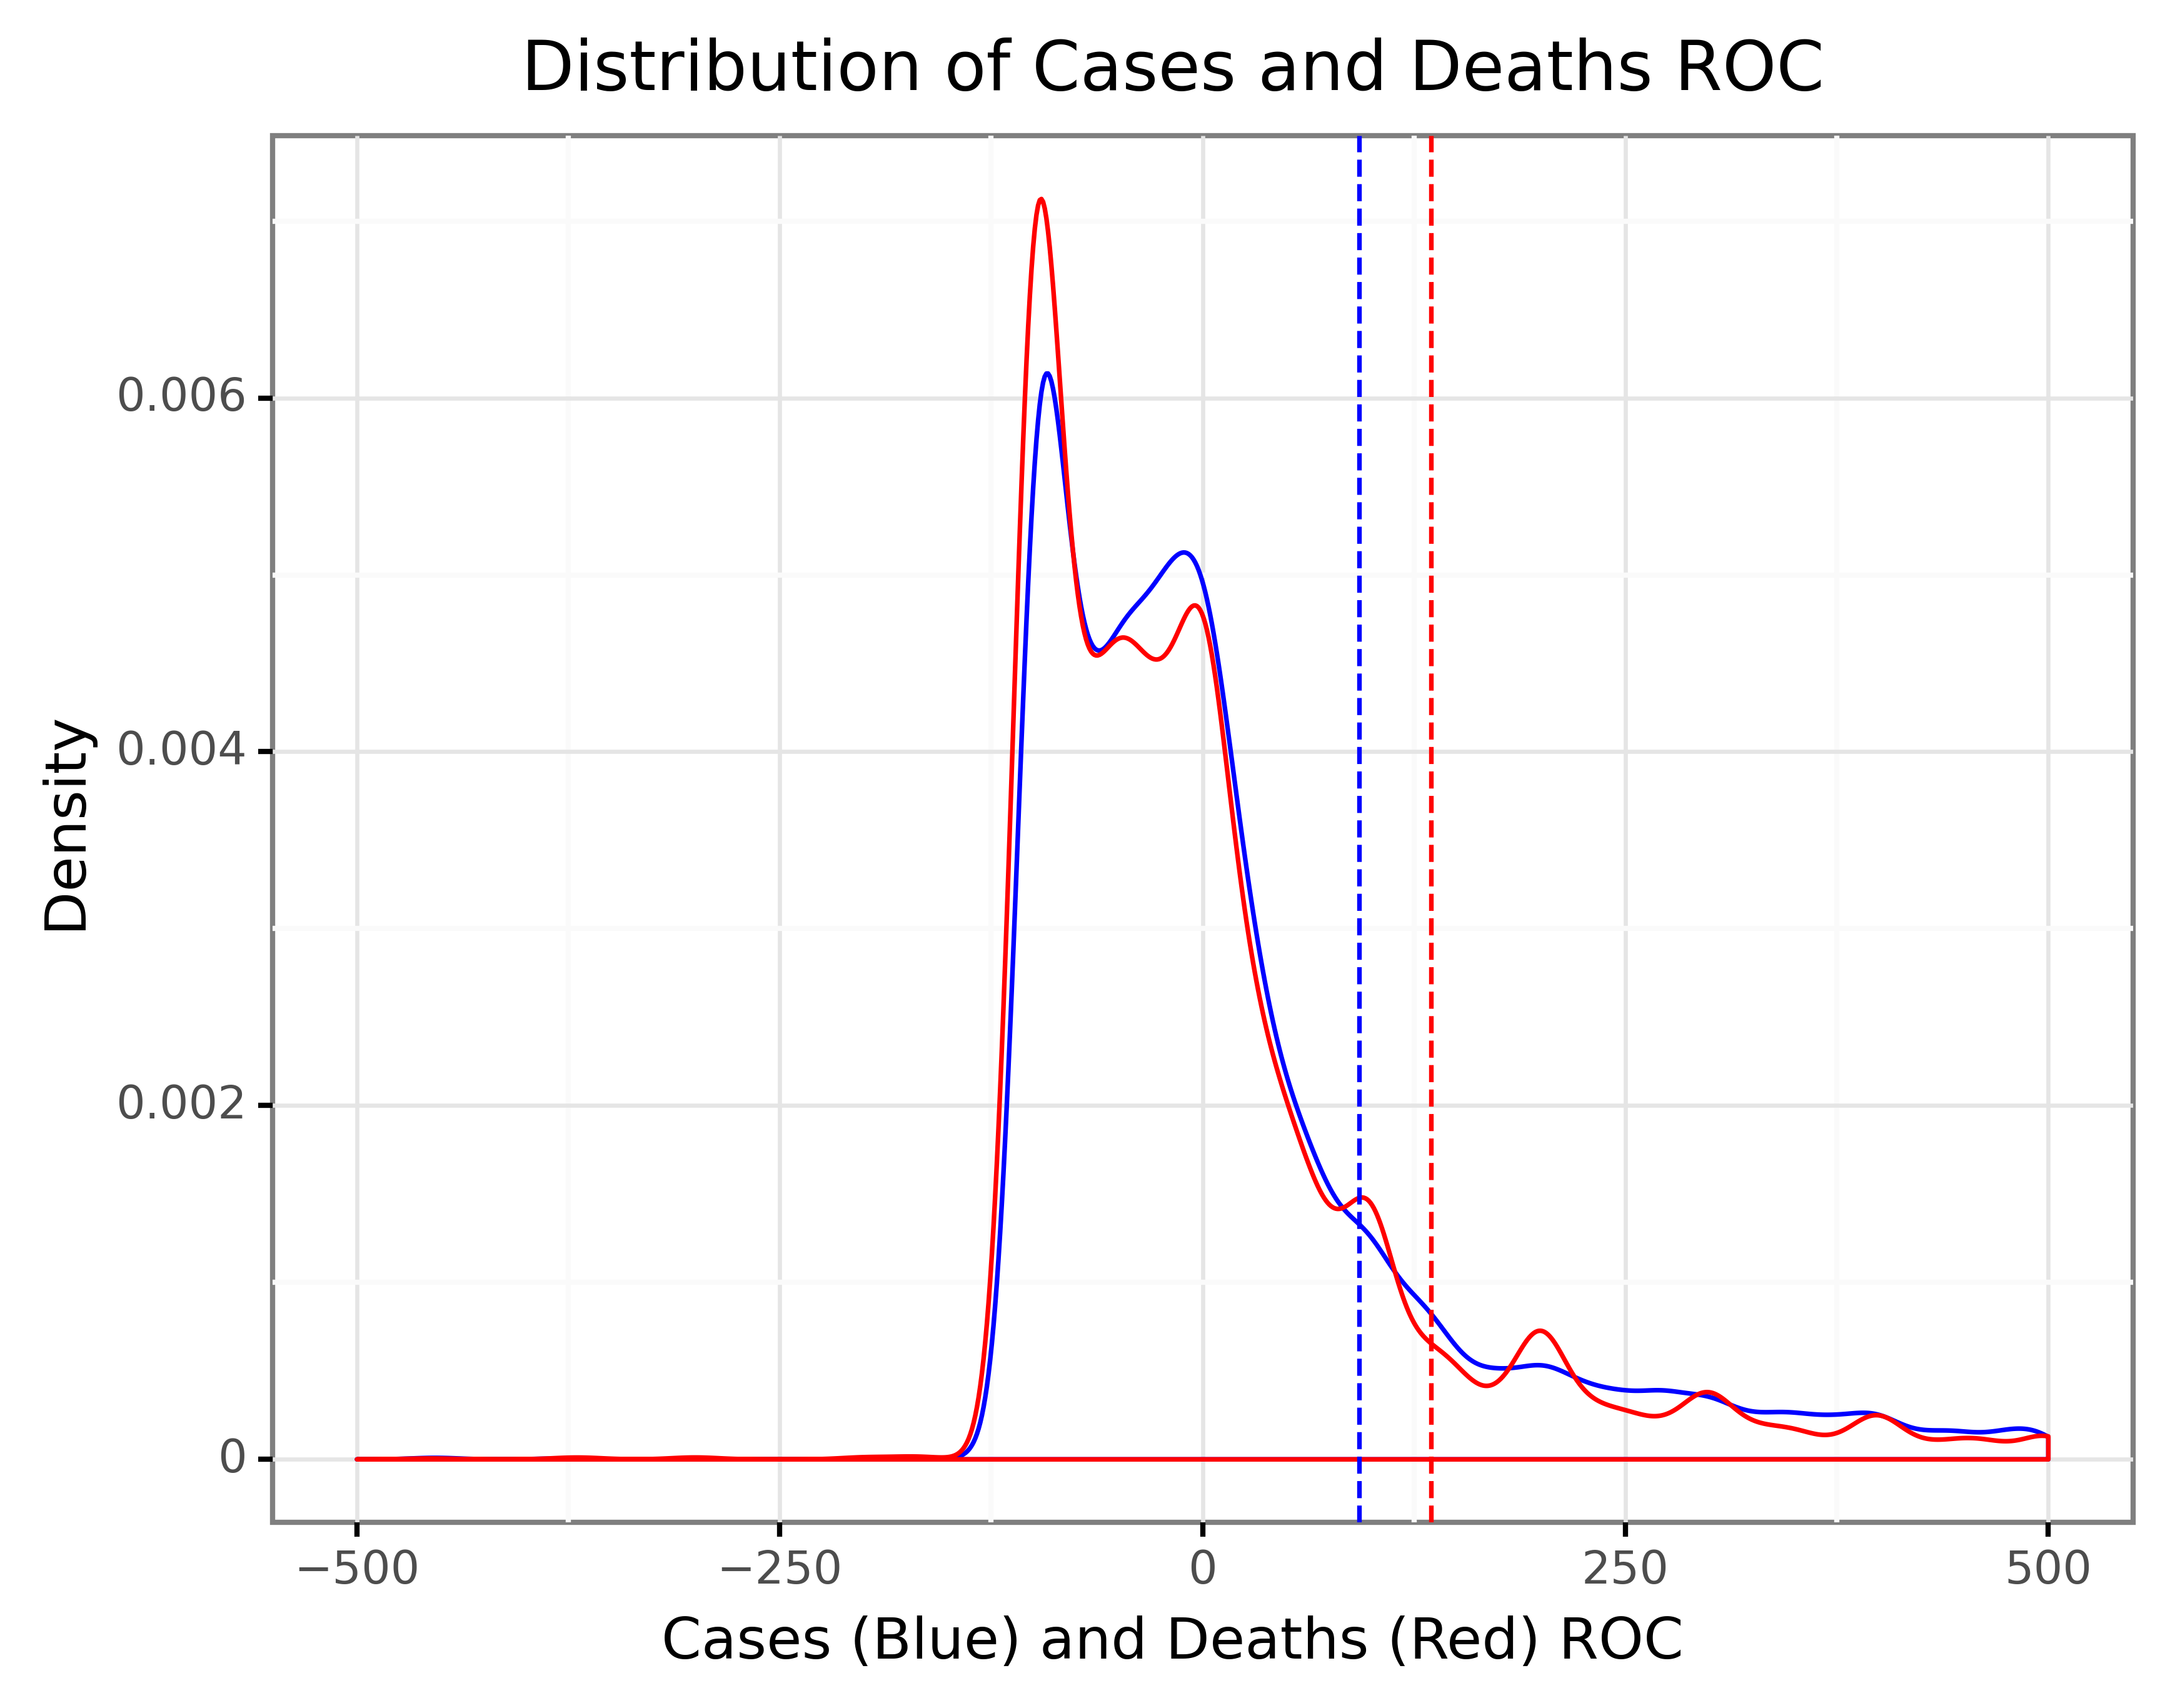
\includegraphics[width= 0.75\linewidth, height= 8cm]{roc_density.png}
    \caption{ROC Distribution Curve}
    \label{fig:my_label}
\end{figure}
Figure 1 displays the ROC’s distribution for weekly cases and deaths. The blue line is the weekly cases, and the red line is weekly deaths. Any negative value in the ROC implies this week’s situation turns better than last week’s. Surprisingly, for both weekly cases and deaths, ROC can be enormous in absolute value. The former is between -1516 and 53300, while the latter is between -300 and 68800. As those extreme values are difficult to make sense of and provide little data information, the project chooses to drop the extreme 1\% in both tails. The dashed lines represent the ROC’s mean after dropping outliers-- weekly cases are 93 and deaths are 135. The existence of negative values makes logged ROC impossible, while absolute values cannot display any information on whether the situation becomes better or worse. Hence, the project codes value larger than the mean as \textit{worse}, implying that within a week period a certain country does a worse job than average. \par 

The remaining processing for \textit{country-week} analysis matches the policy with the week number. The project codes 1 in \textit{active\_policy} for any week within the span of an effective policy and creates an ordinal variable \textit{compliance\_ordinal} from 1 to 4 (1-voluntary, 2-mandatory, 3-mandatory with fines, and 4-mandatory with jail) dummy variables for policy types. \par 

After the pre-processing, the project takes the (supervised) machine learning techniques to discover which variables are pivotal to affect the ROC. Supervised learning helps figure out how to predict the outcome of interest (ROC) from several key variables of interest illustrated above. Since the outcome variable is binary, the project specifically employs \textit{naive Bayes}, \textit{k-nearest neighbors}, \textit{decision tree}, and \textit{random forest decision} algorithm. Based on Bayes' theorem, \textit{Naive Bayes} is to select the most probable outcome based on the newly added features. \textit{K-NN} is based on k nearest data points to predict the outcome. \textit{Decision tree} is useful to predict the outcome where features might interact with each other. \par

In parallel with machine learning, the project would take the traditional regression analysis to understand how the public health infrastructure’s proxy variables could affect cases, deaths, and tests. All three model control for the \text{GDP per capita} and \text{logged inbound visitors}. In addition, because of the potential distortion of insufficient testings, the project chooses to create the case-test and death-test ratio is to substitute for the cases and deaths per thousand people. All estimates are based on the ordinary least square approach. 


\section*{Results}
\begin{figure}[h]
\begin{subfigure}{0.5\textwidth}
  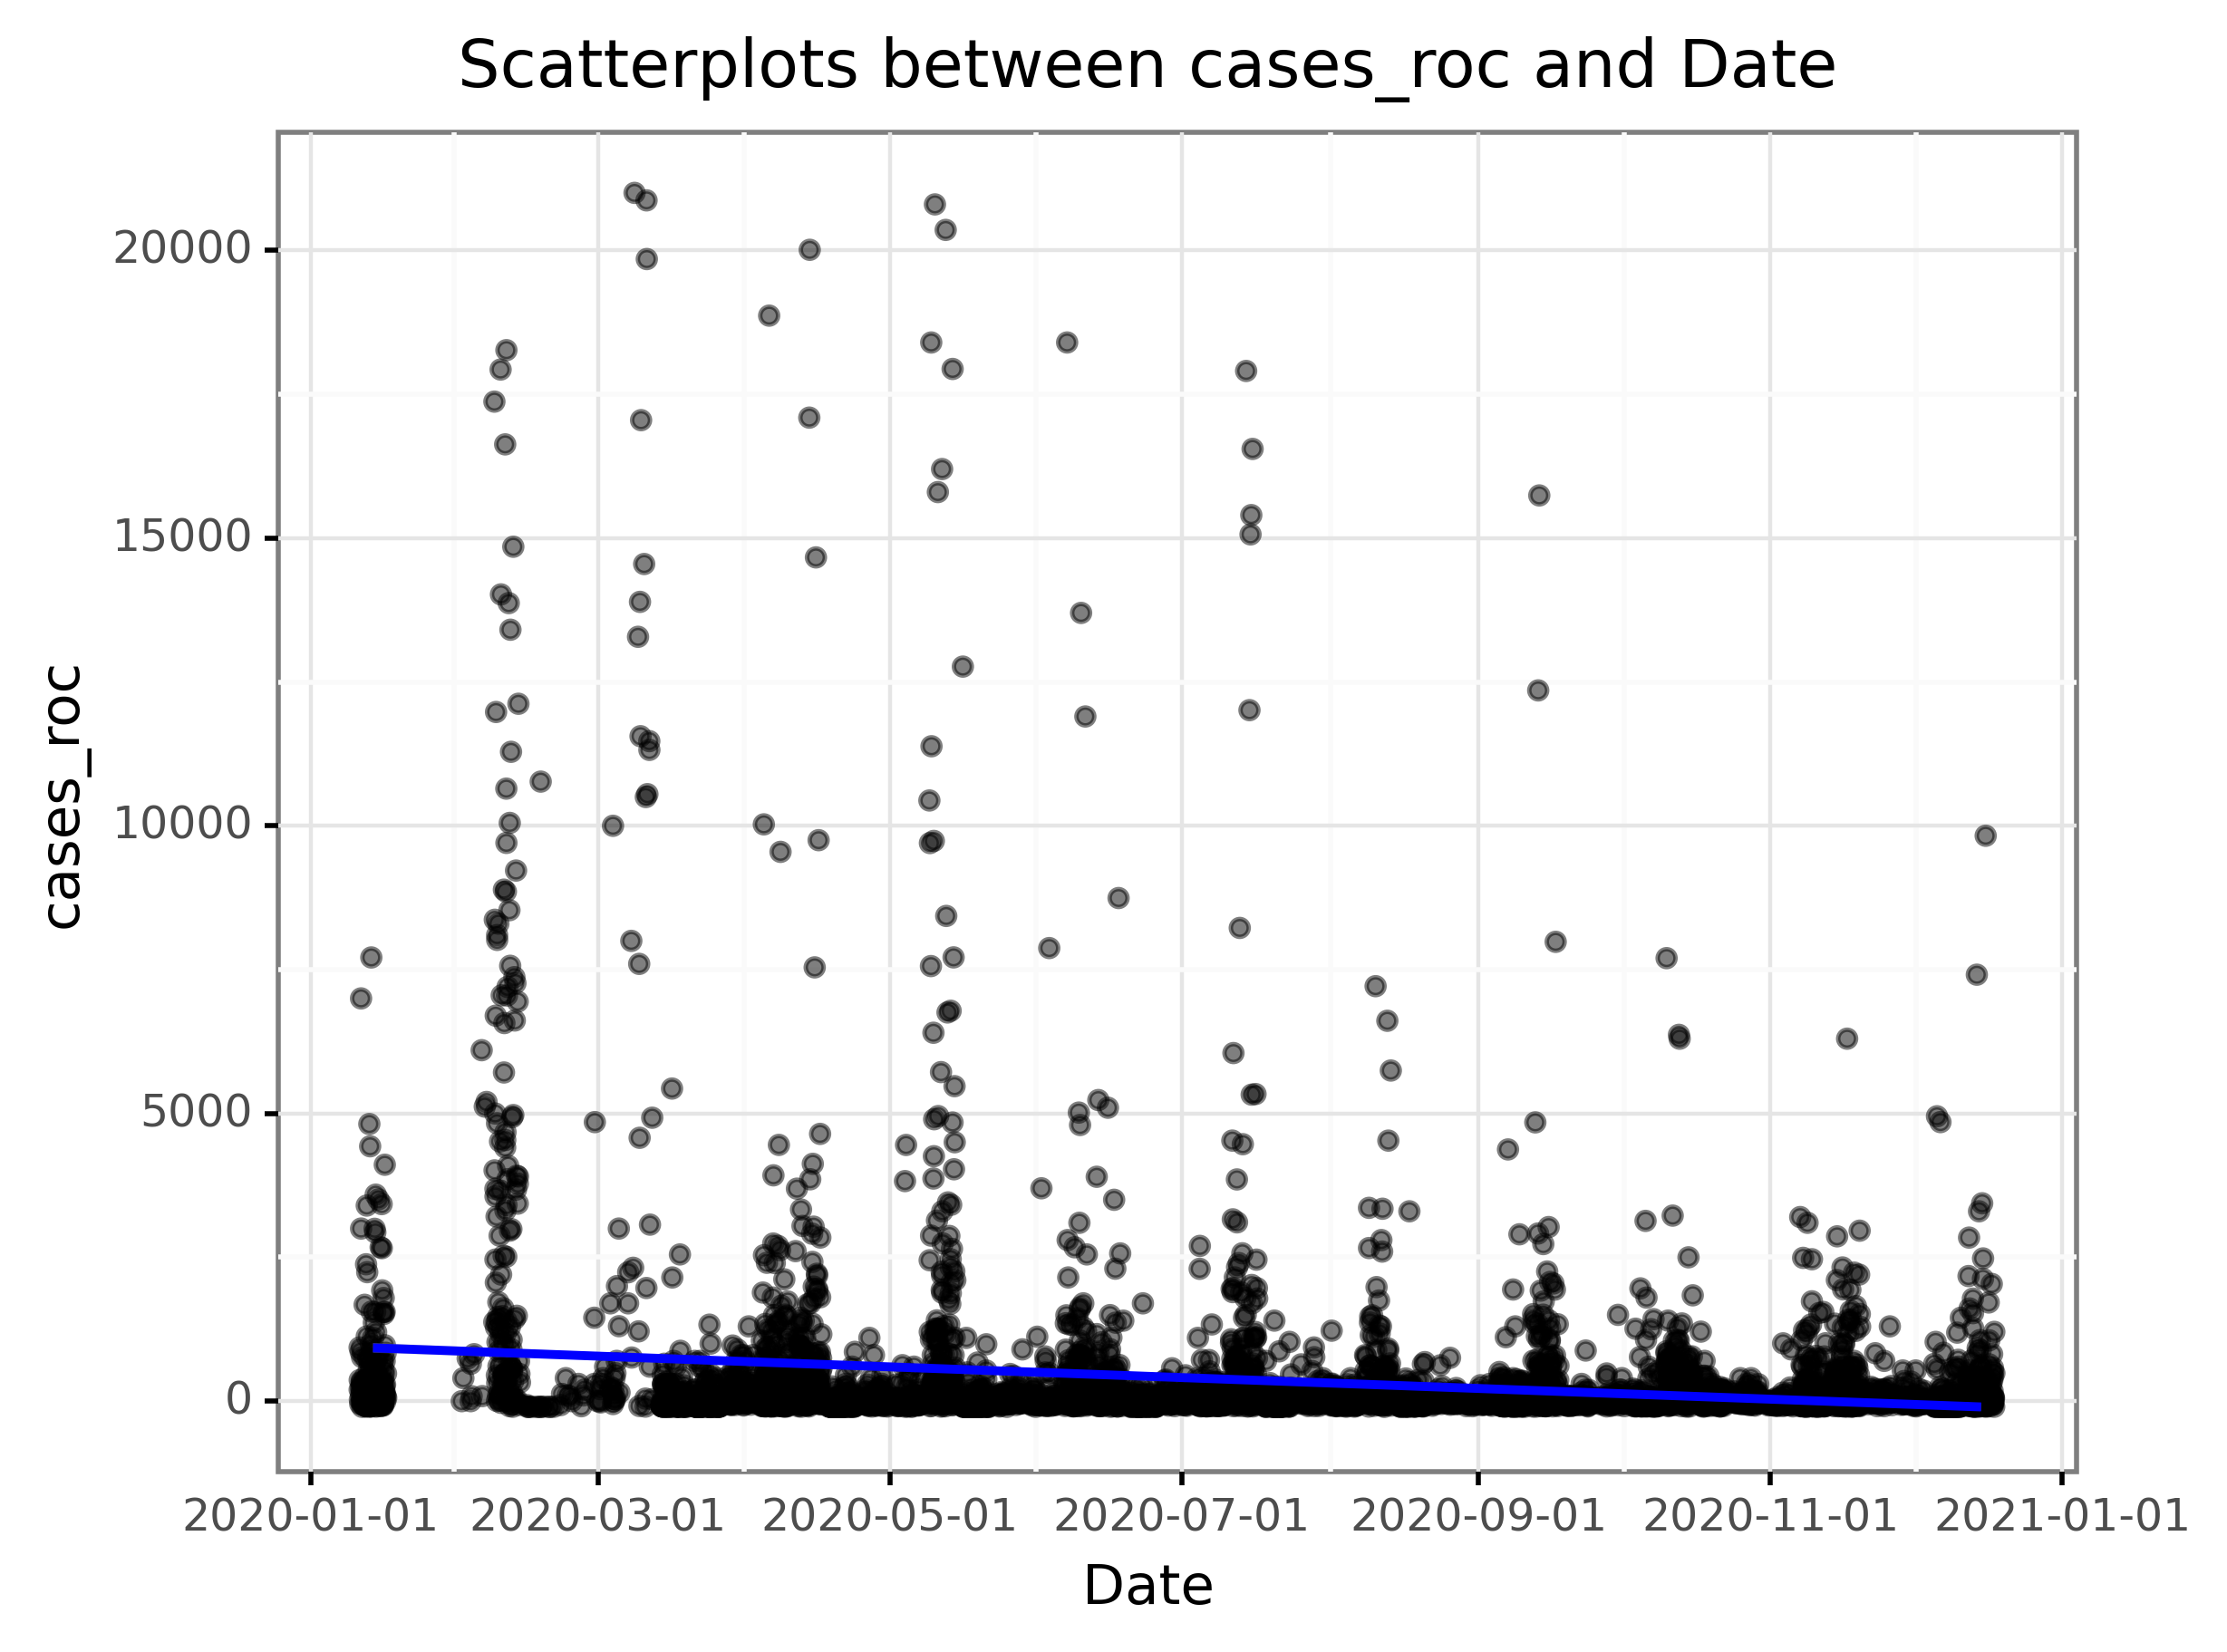
\includegraphics[width=\linewidth, height= 8cm]{cases_rocplot.png}
  \caption{Cases ROC}
  \label{fig:subim1}
\end{subfigure}
\begin{subfigure}{0.5\textwidth}
  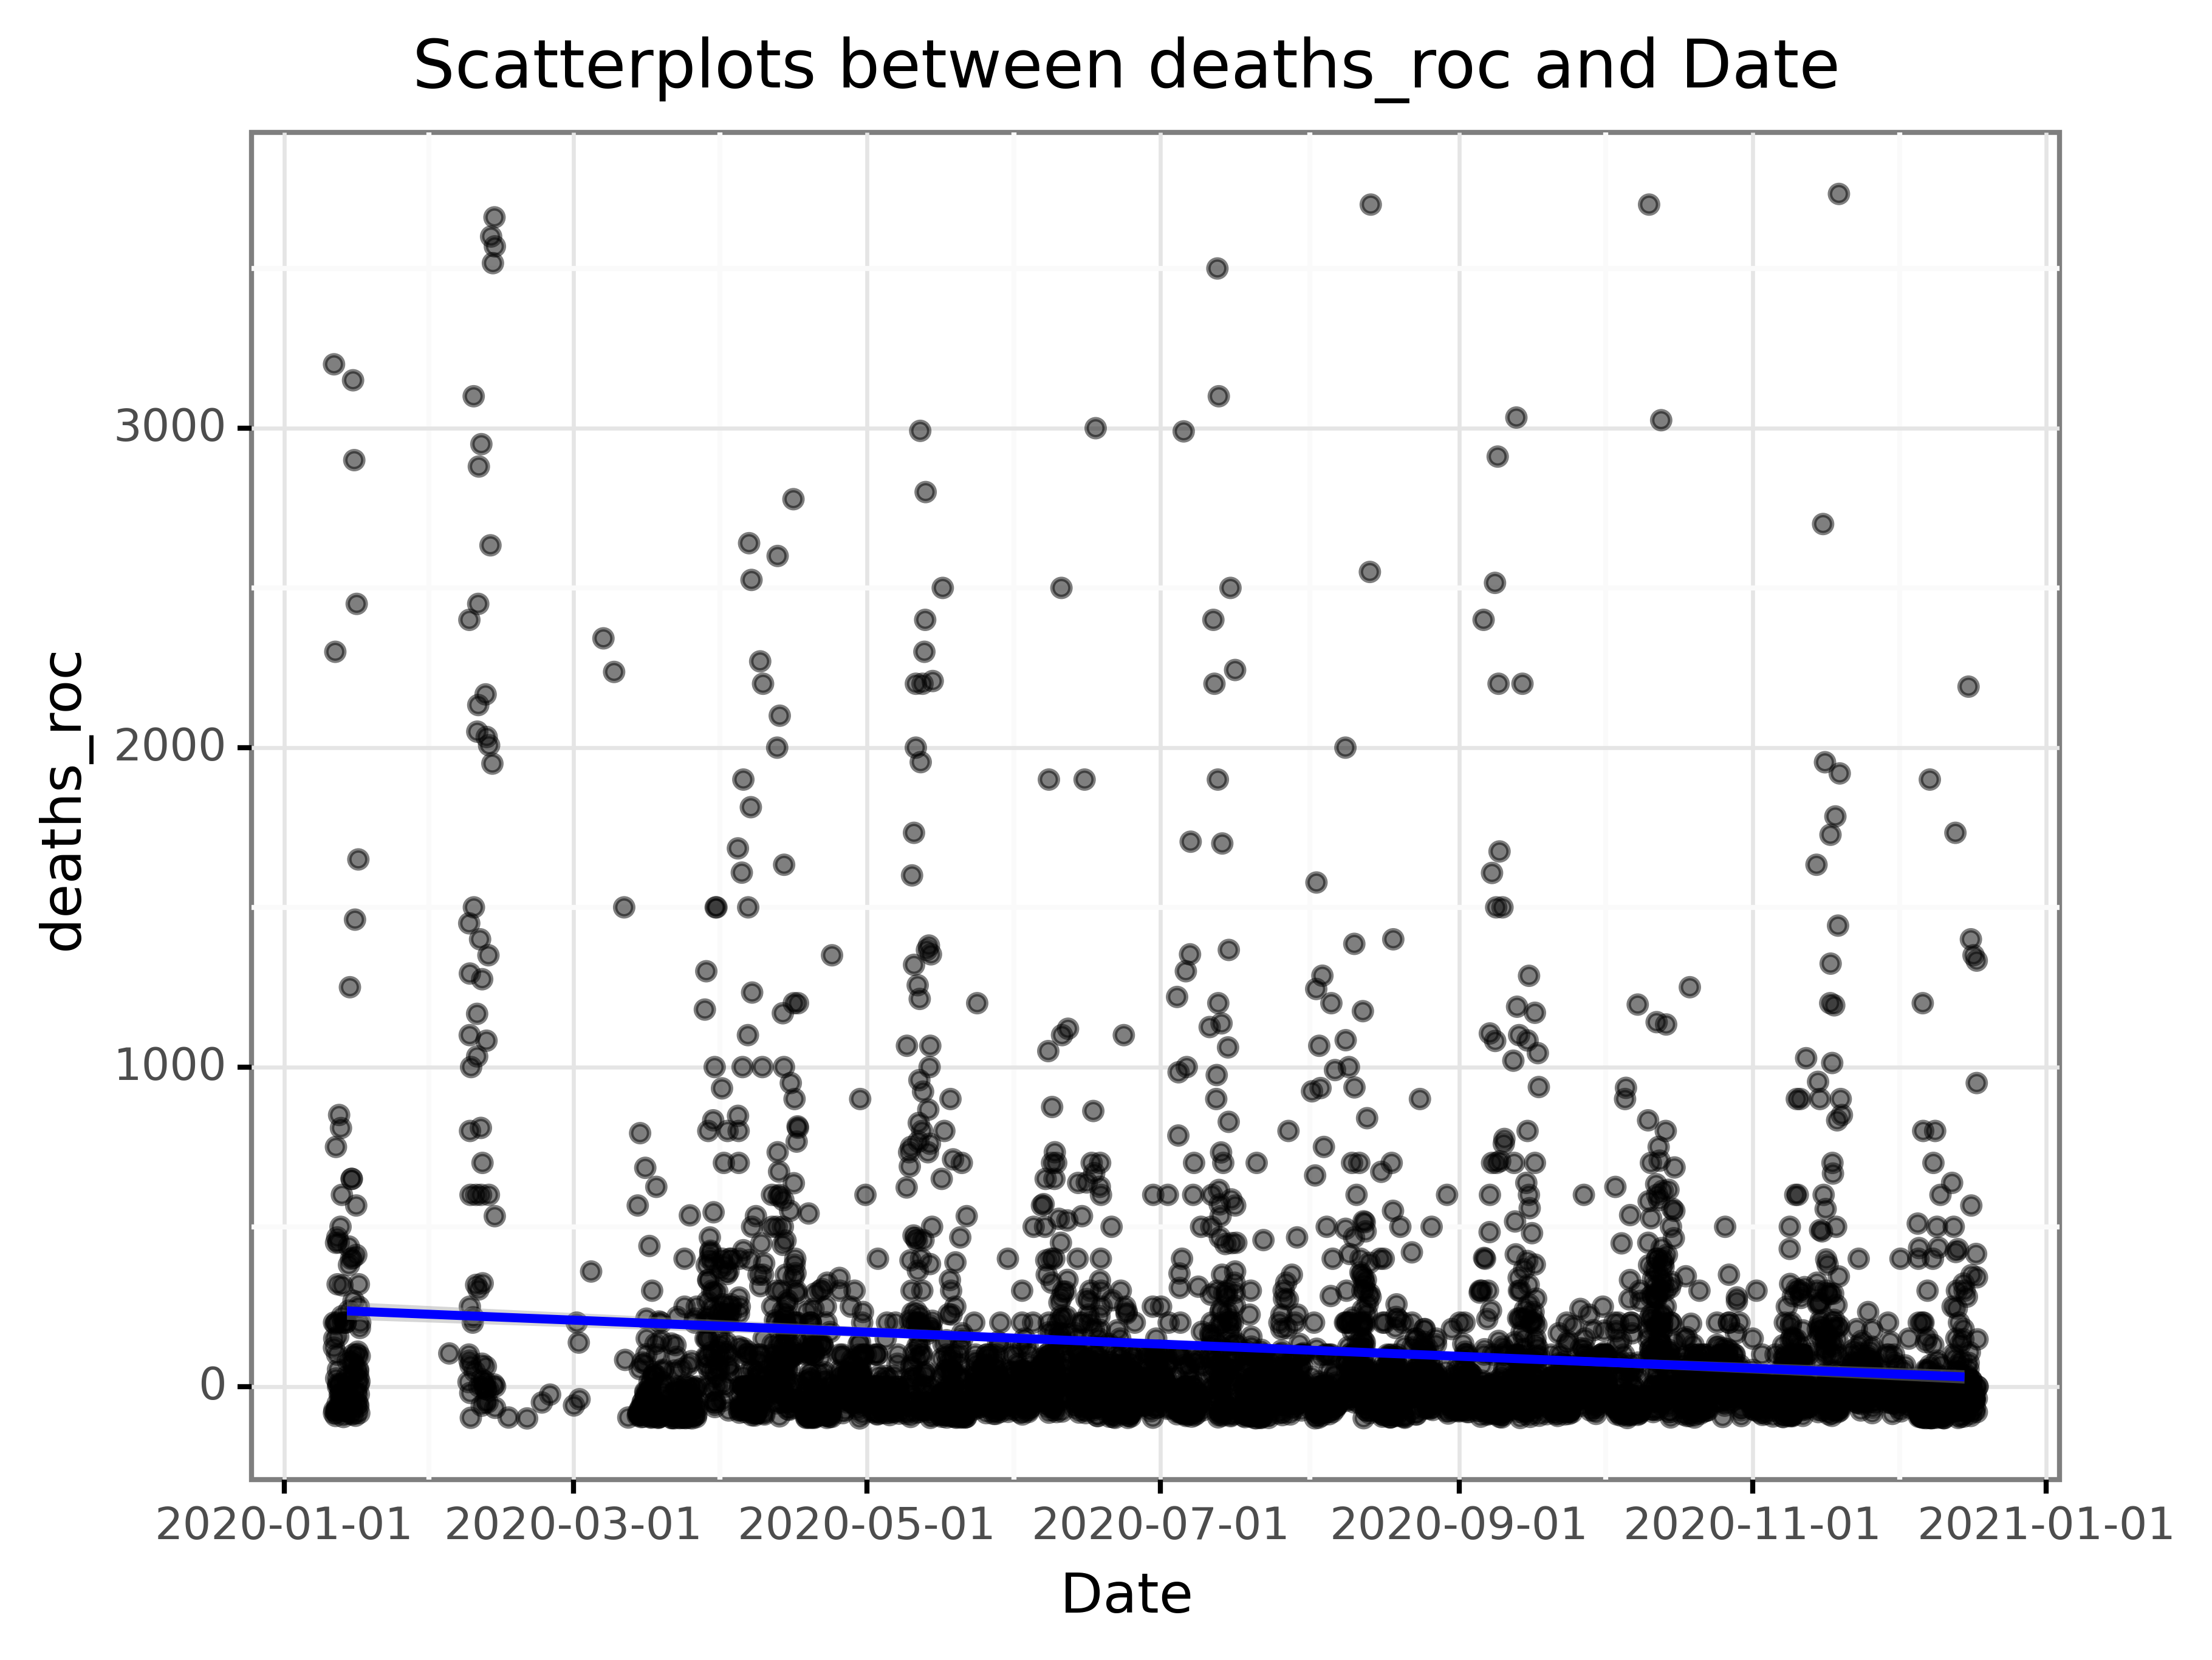
\includegraphics[width=\linewidth, height= 8cm]{deaths_rocplot.png}
  \caption{Deaths ROC}
  \label{fig:subim2}
\end{subfigure}
\caption{Relationship Between ROC and Date}
\label{fig:image2}
\end{figure}
Before any sophisticated results, figure 2 displays the relationship between ROCs and dates. As time goes on, we can see a \textit{seemingly} decreasing trend reflected by the blue line in both ROC scatterplots. After a more cautious look, it appears that in ROC for weekly cases, points are scattered more densely from September than before, while points in ROC for deaths fall into a relatively stable interval. These results are consistent with the initial high reproduction number and relatively low fatality rate compared to other infectious respiratory diseases. What’s more, one can observe points are more likely to stay at a high level between February and May, and it also fits the worldwide first wave outbreak.\par 
\begin{figure}
    \centering
    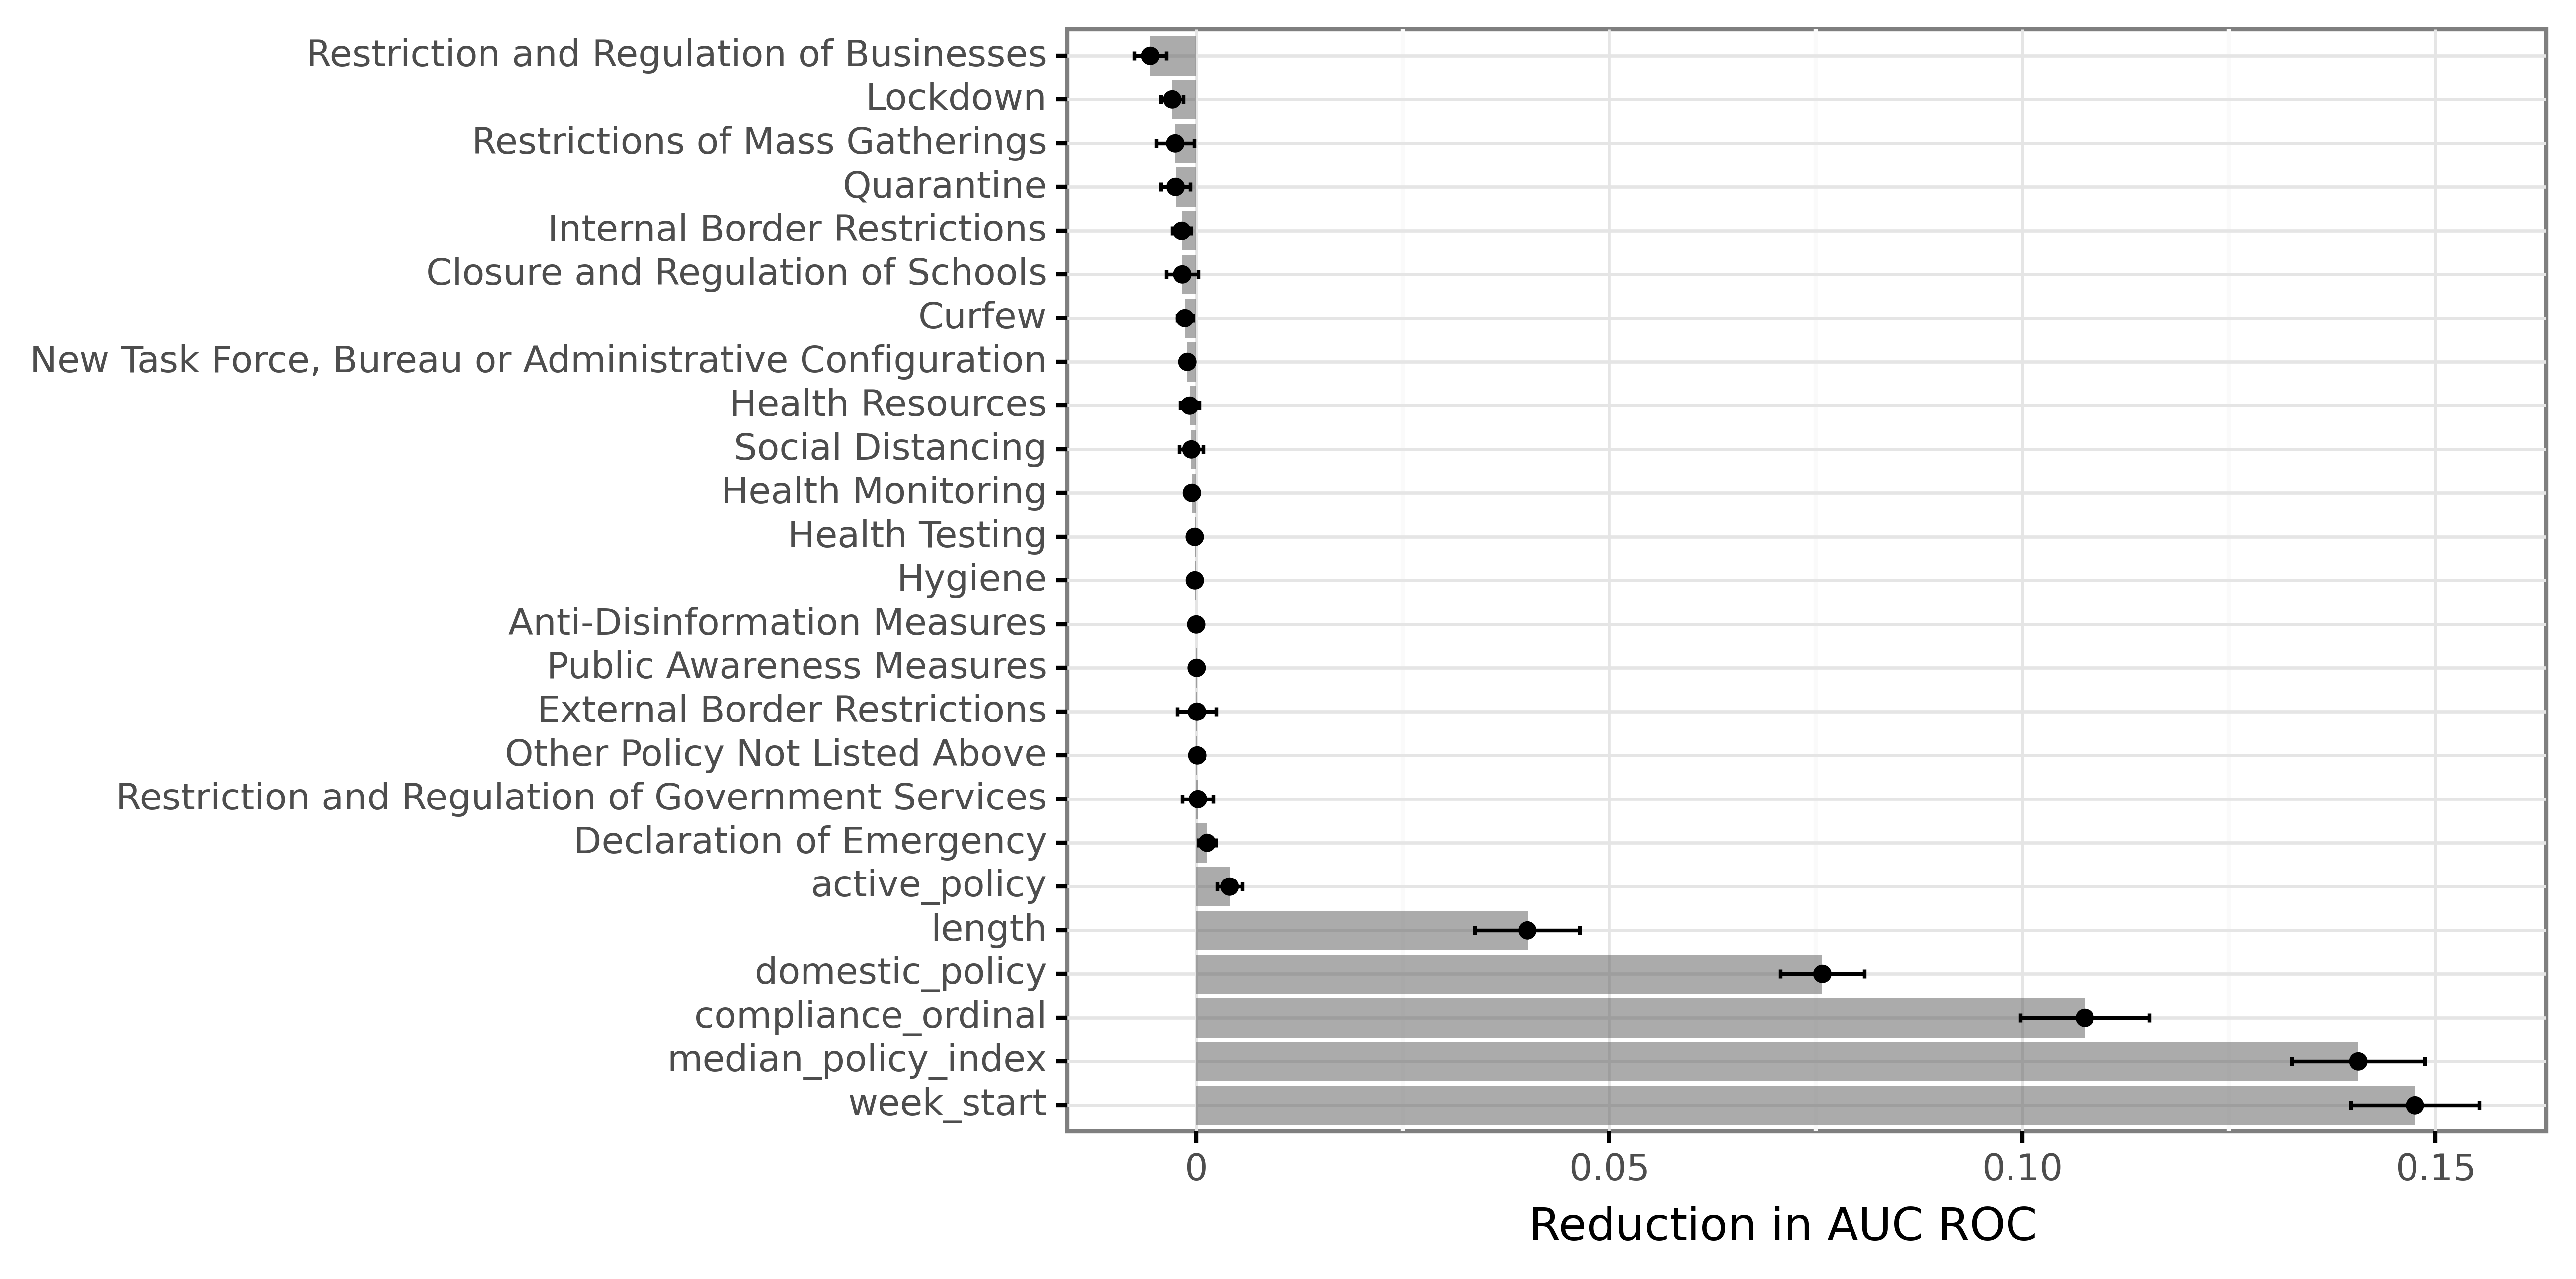
\includegraphics[width= 0.8\linewidth, height= 8cm]{cases_auc_roc.png}
    \caption{Variable Importance}
    \label{fig:my_label}
\end{figure}
Turning to the machine learning results on ROC for weekly cases, the best method to predict is \textit{k-NN} with $k=5$ with the Area Under Curve (AUC) score is 0.888. AUC score reflects the model’s predictivity, and 0.50 in AUC is equivalent to a random draw. A higher score implies a better model, and a model with a score above 0.8 is useful for predicting. Figure 2 displays each feature’s permutation importance after repeating 25 times. The larger the score is, the more critical that feature would be in deciding whether next week’s situation would worsen. The top five features include \textit{starting week}, \textit{policy activity score}, and \textit{compliance level}. Although \textit{starting week} could be a tricky feature to remain in the model, it indirectly reflects the importance of acting quickly.  Figure 4a) appears to confirm the argument, and there is a steadily decreasing trend before week 12 (before March 22) and a sudden increase in the next few weeks. However, that relationship could be spurious since late March happened to be the first wave of pandemics worldwide.\par 

\begin{figure}[h]
\begin{subfigure}{0.5\textwidth}
  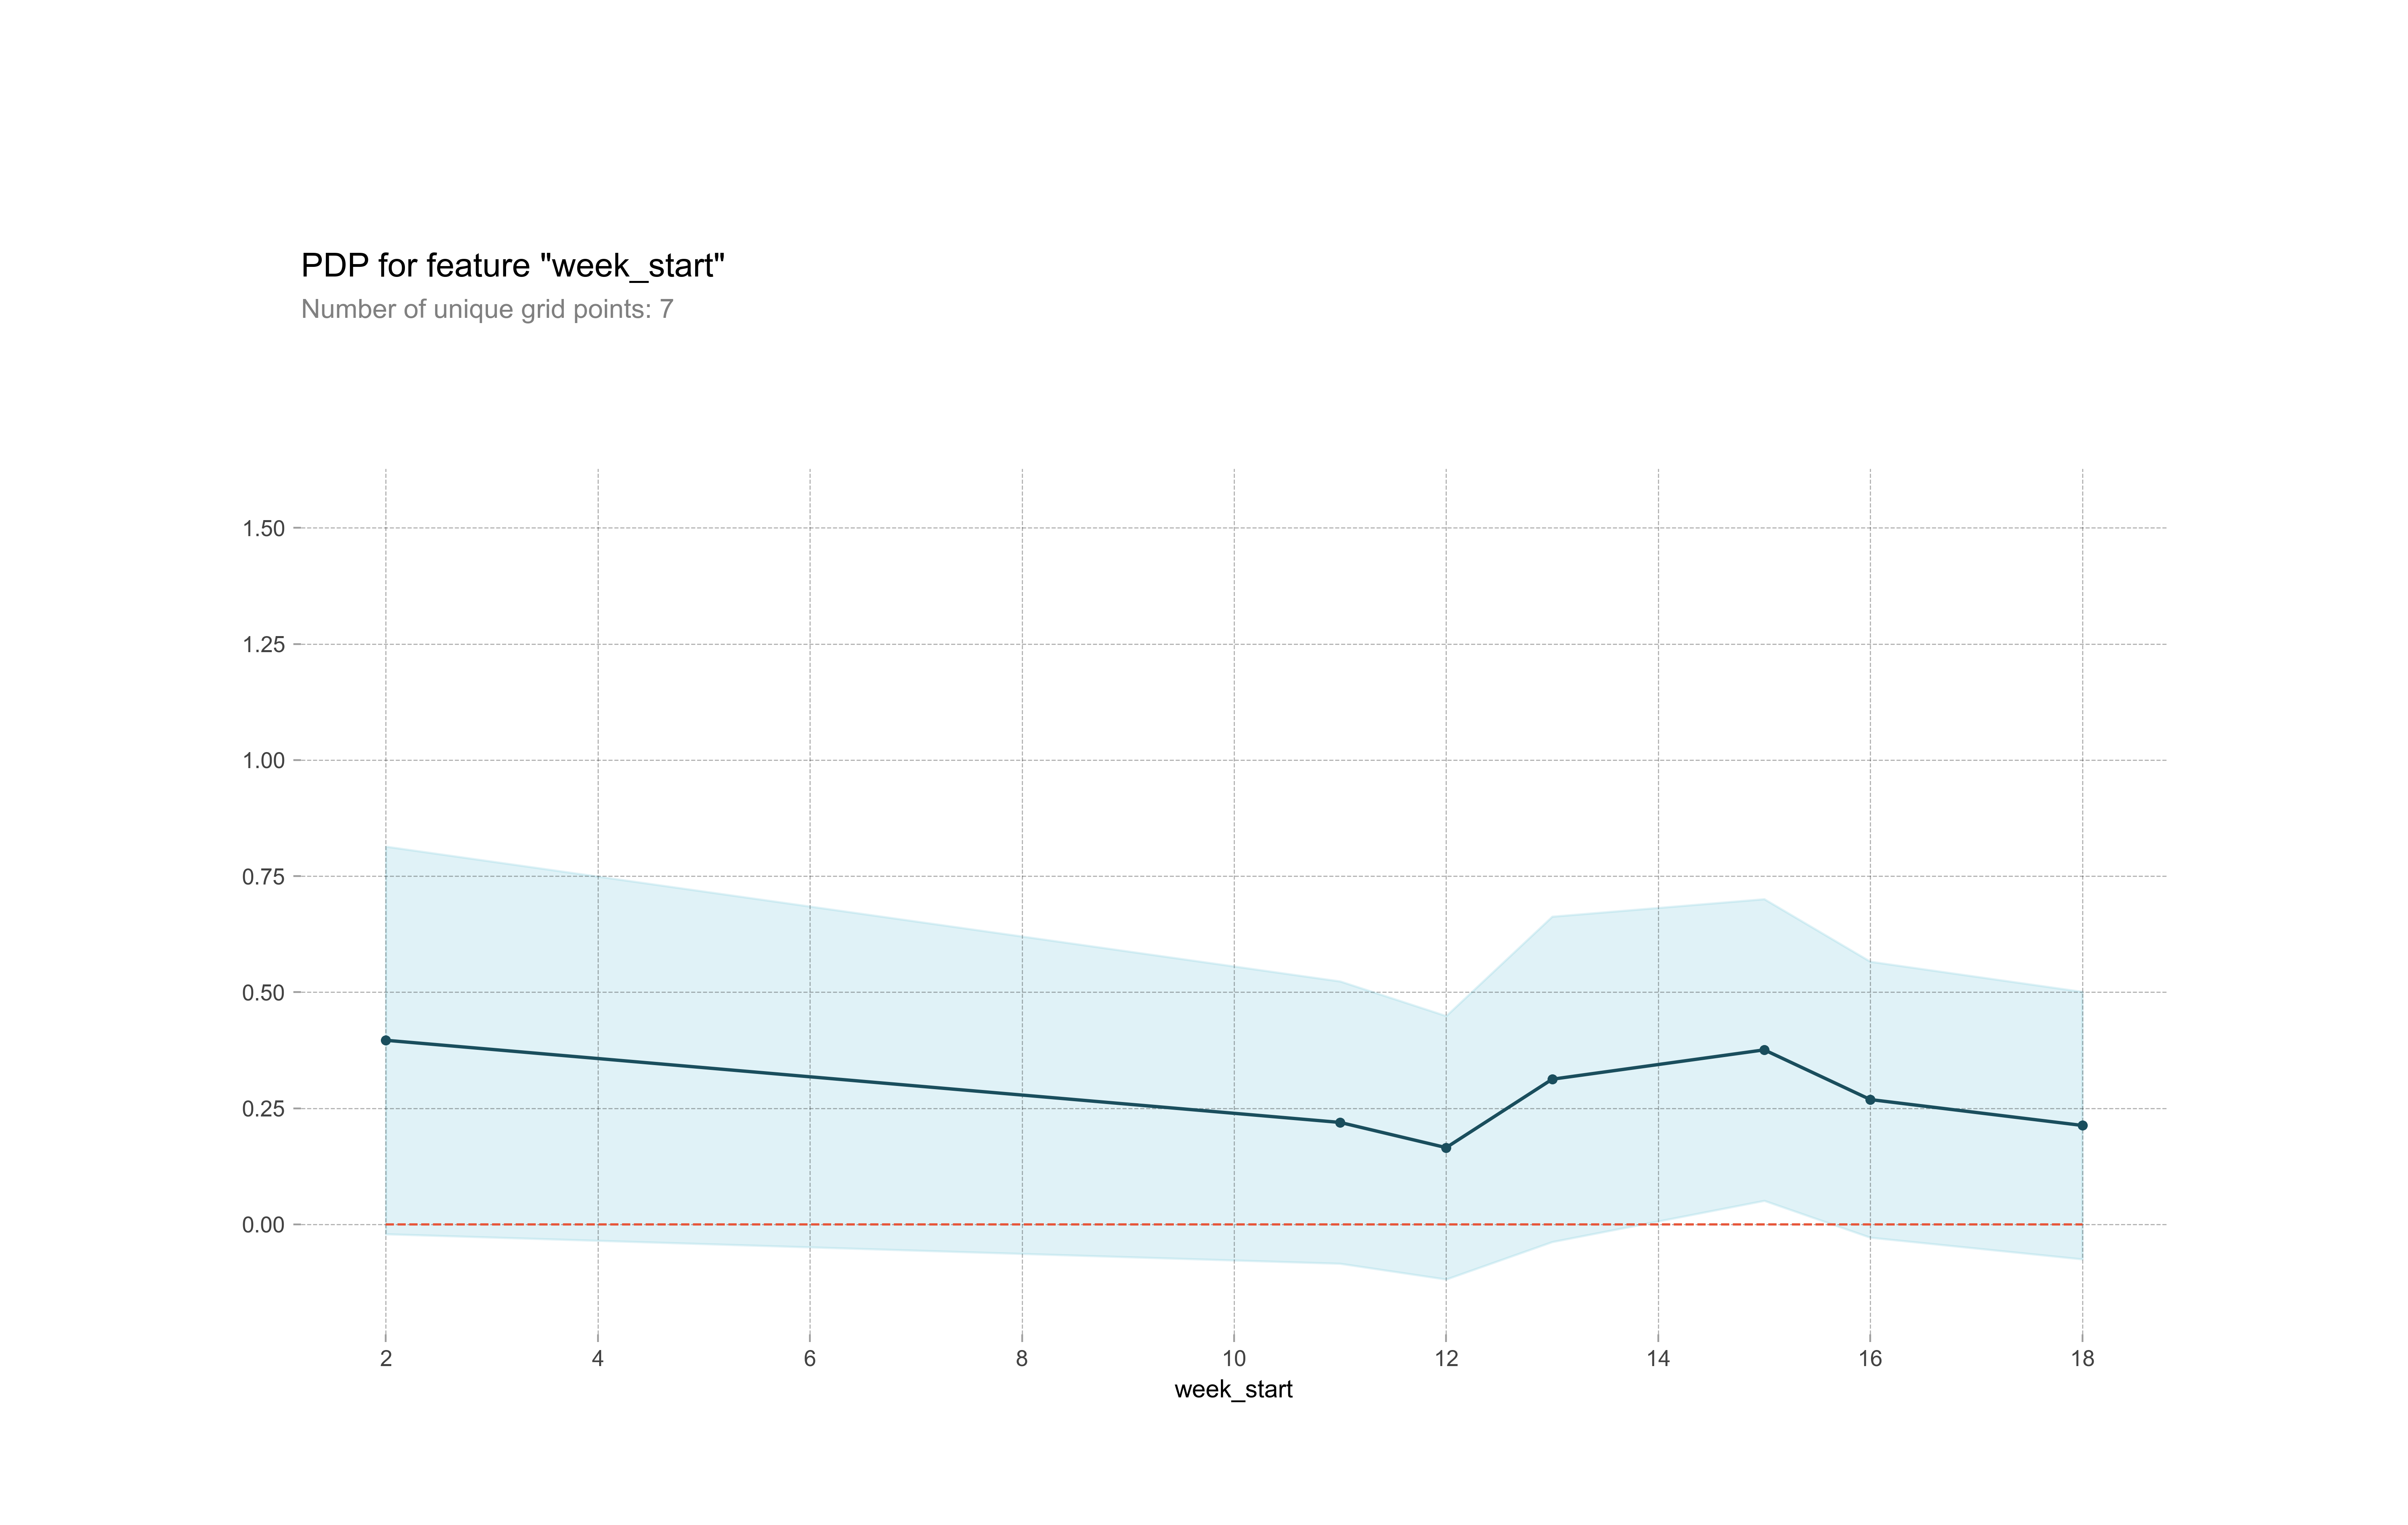
\includegraphics[width=\linewidth, height= 8cm]{pdp_plot_week_start.png}
  \caption{PDP for Starting Week}
  \label{fig:subim1}
\end{subfigure}
\begin{subfigure}{0.5\textwidth}
  \includegraphics[width=\linewidth, height= 8cm]{pdp_plot_compliance.png}
  \caption{PDP for Compliance}
  \label{fig:subim2}
\end{subfigure}
\caption{Partial Dependence Plots}
\label{fig:image2}
\end{figure}

The second most important feature, \textit{policy activity score}, is an index created by \textit{CoronaNet Research Project} to measure the policy activity. Since it is already an aggregate index after treatment, it becomes less fruitful to examine its importance. \textit{Compliance} is the third most important feature. Figure 4b) shows that if a policy starts from voluntary to normal mandatory level, it will negatively affect ROC for weekly cases, implying the situation turns better. Yet, once a policy is compulsory, additional punishments (fines or jail time) will not positively affect the situation. That phenomenon is consistent with common sense. Other top features, like \textit{domestic policy} or \textit{length}, seem not to produce observable differences on the plot.\par 
\begin{figure}
    \centering
    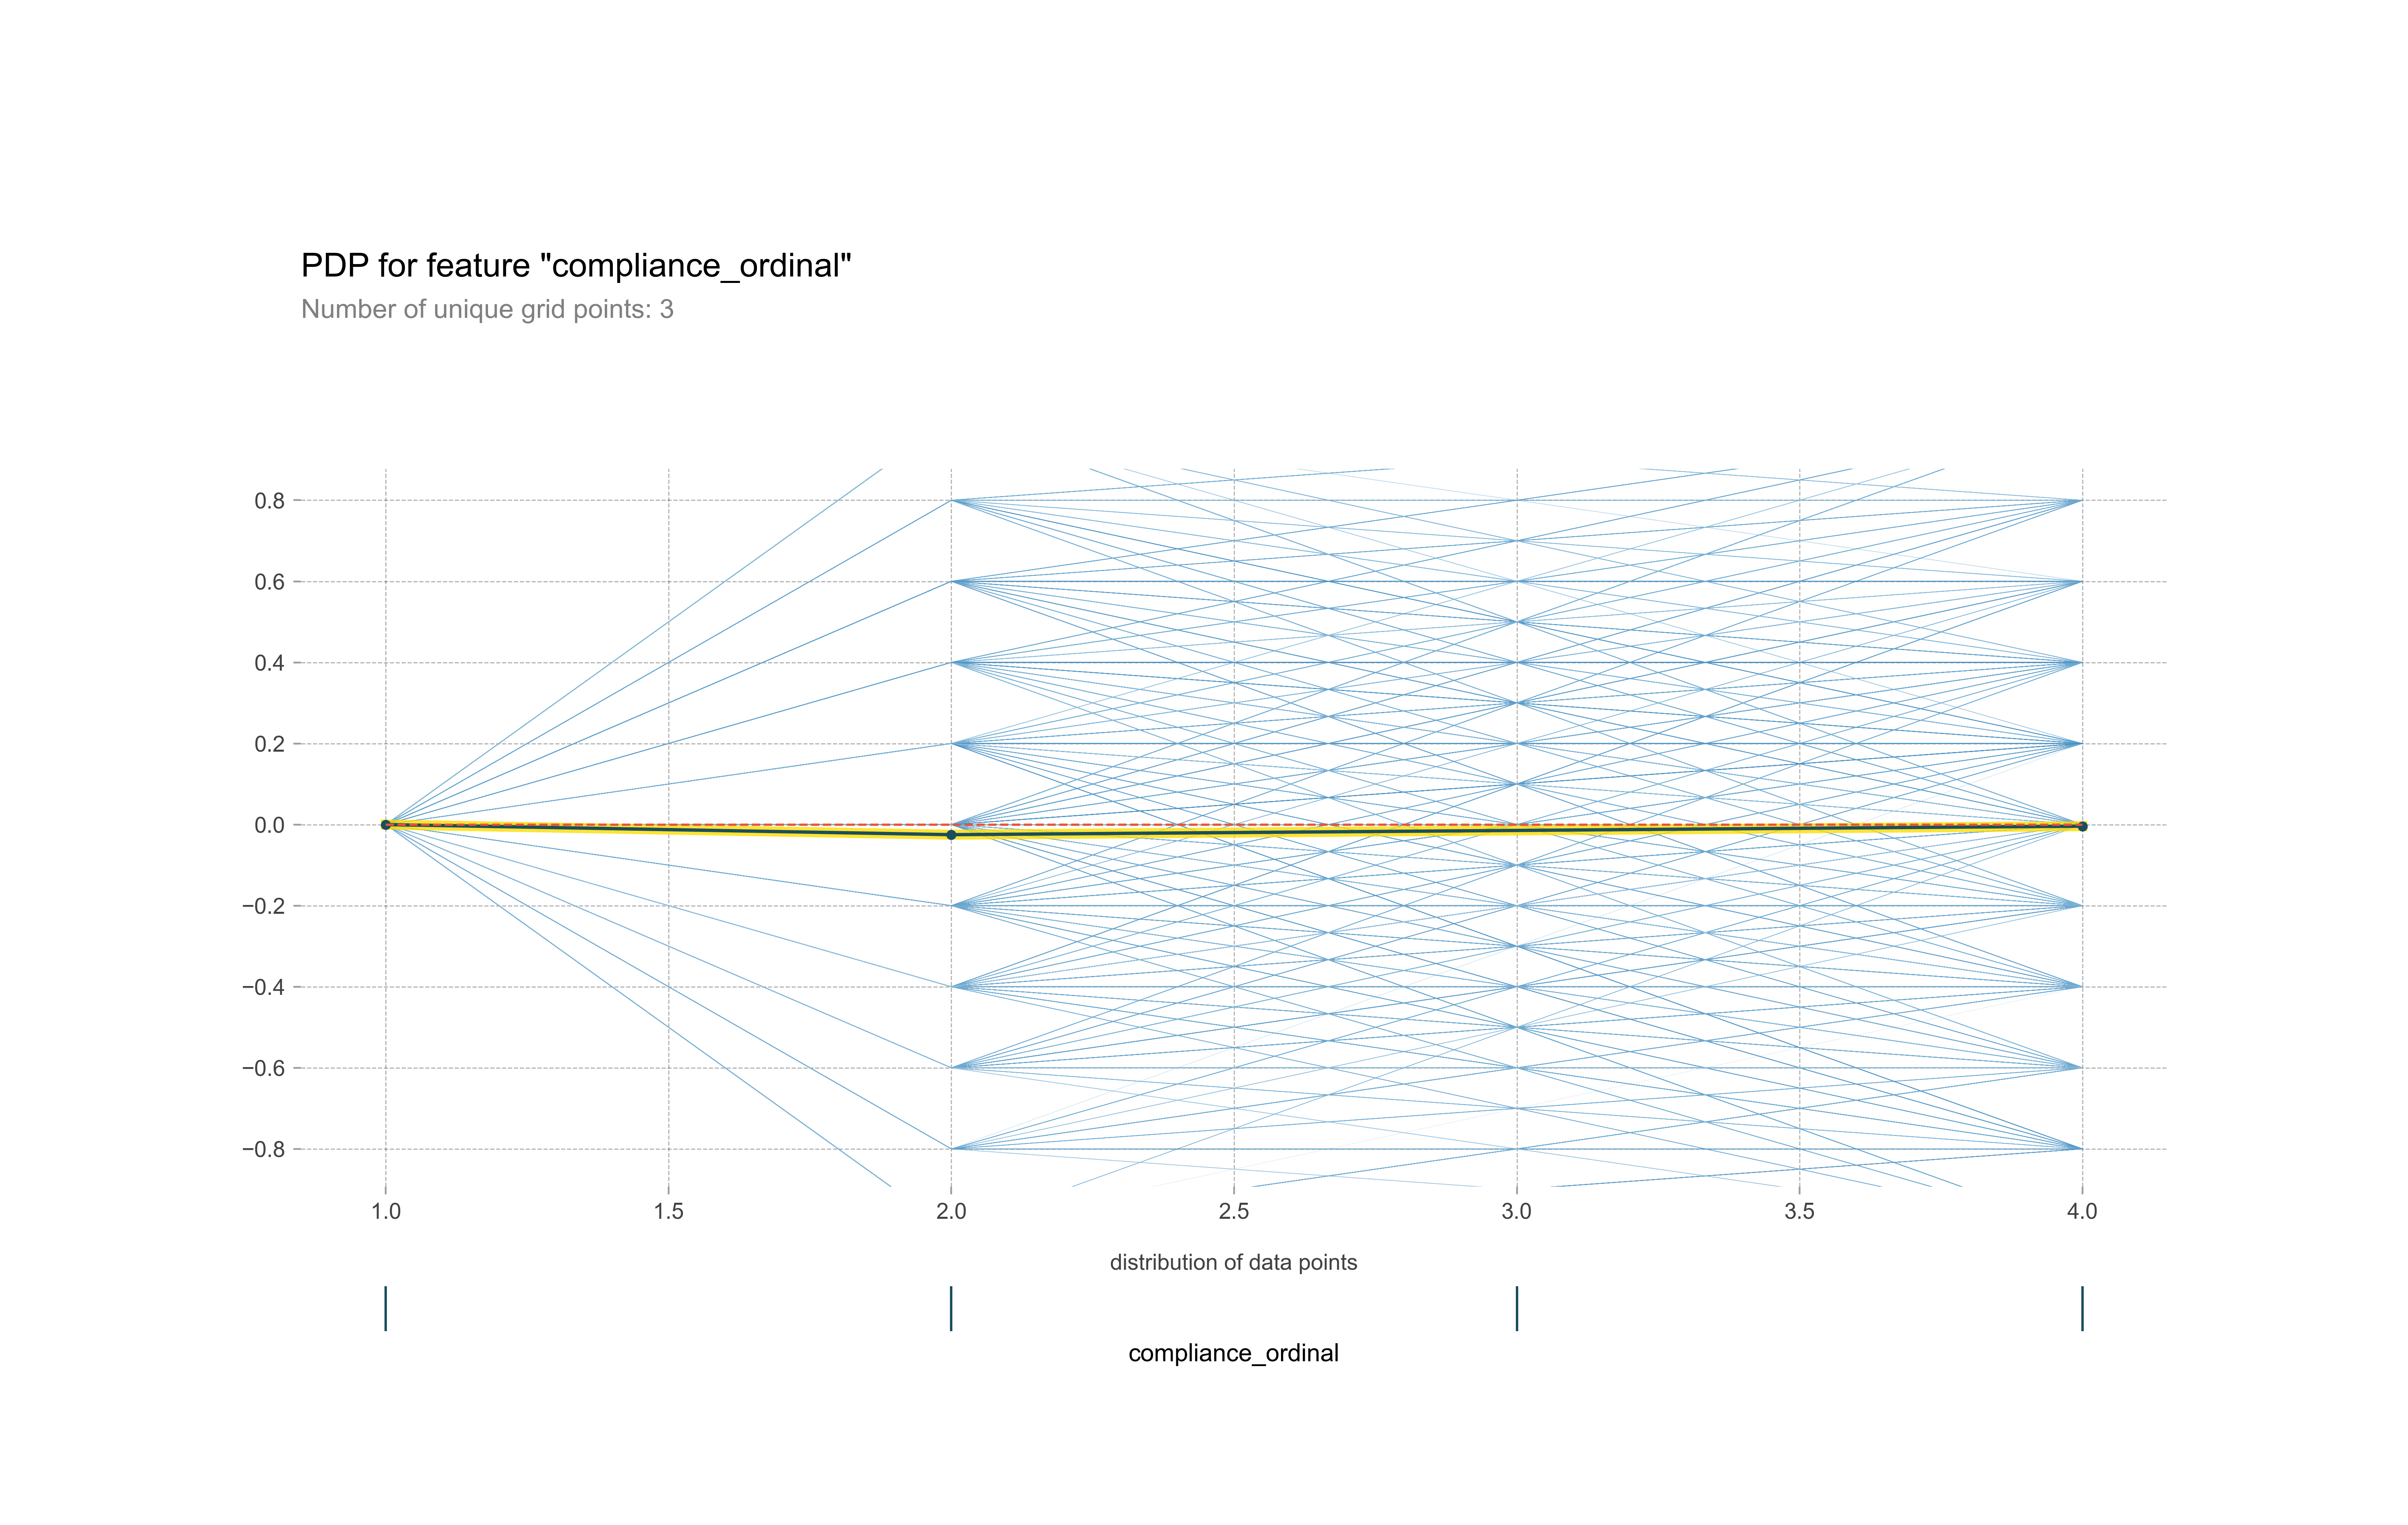
\includegraphics[width= 0.6\linewidth, height= 6cm]{compliance_ordinal_iceplot.png}
    \caption{Individual Conditional Expectation (ICE) Plot}
    \label{fig:my_label}
\end{figure}
Figure 5 represents compliance’s Individual Conditional Expectation (ICE) plot, where each ICE line represents an instance given the change of one feature. The inconsistent lines with a one-unit increase in compliance level imply the heterogeneous effects by interactions or paths resulting from the specific country features. The particular paths raise the possibility of the latter explanation. Meanwhile, the average ICE (PDP) is still useful to capture what would happen in a general situation, instead of any specific country. \par 

Beyond machine learning, the project runs the regression analysis on cases, deaths, and tests, and the result is shown in Table 1. Starting from column 3, it is understandable that proxy variables of the public health infrastructure, \textit{health expenditure per capita} and \textit{immunization ratio}, exert positive effects on \textit{test per 1k}. Originally, when directly running regressions on cases and deaths, both coefficients on logged GDP per capita were positive, and one was not statistically significant. After considering the potential under-testing and creating the ratio as dependent variables, both coefficients turn negative, implying that the increase in GDP per capita is associated with decreasing cases and deaths. Moreover, the increase in hospital beds per thousand population or immunization ratio is associated with the decreasing death-test ratio, which is understandable considering the ventilator’s need for critical cases. In short, a strong health infrastructure seems more relevant to deaths and tests. \par
 

\begin{table}[!htbp] \centering 
  \caption{Results} 
  \label{} 
\begin{tabular}{@{\extracolsep{5pt}}lD{.}{.}{-3} D{.}{.}{-3} D{.}{.}{-3} } 
\\[-1.8ex]\hline 
\hline \\[-1.8ex] 
 & \multicolumn{3}{c}{\textit{Dependent variable:}} \\ 
\cline{2-4} 
\\[-1.8ex] & \multicolumn{1}{c}{Case-Test Ratio} & \multicolumn{1}{c}{Death-Test Ratio} & \multicolumn{1}{c}{Tests per 1k} \\ 
\\[-1.8ex] & \multicolumn{1}{c}{(1)} & \multicolumn{1}{c}{(2)} & \multicolumn{1}{c}{(3)}\\ 
\hline \\[-1.8ex] 
 Visitor (log) & 0.003 & 0.0002 &  \\ 
  & (0.003) & (0.0001) &  \\ 
  & & & \\ 
 GDP per capita (log)  & -0.061^{*} & -0.003^{**} & 31.483^{**} \\ 
  & (0.035) & (0.002) & (15.866) \\ 
  & & & \\ 
 Health per capita (log) & 0.015 & 0.002 & 45.928^{***} \\ 
  & (0.028) & (0.001) & (15.943) \\ 
  & & & \\ 
 Hospital Bed per 1k & -0.008 & -0.0005^{*} & -10.523 \\ 
  & (0.006) & (0.0003) & (8.398) \\ 
  & & & \\ 
 Life expectancy & 0.006 & 0.0002 & 3.675^{**} \\ 
  & (0.004) & (0.0002) & (1.800) \\ 
  & & & \\ 
 Immunization Ratio (DPT) & -0.002 & -0.0001^{**} & -0.308 \\ 
  & (0.001) & (0.0001) & (1.264) \\ 
  & & & \\ 
 Constant & 0.325 & 0.016 & -613.857^{***} \\ 
  & (0.250) & (0.011) & (154.265) \\ 
  & & & \\ 
\hline \\[-1.8ex] 
Observations & \multicolumn{1}{c}{103} & \multicolumn{1}{c}{103} & \multicolumn{1}{c}{186} \\ 
R$^{2}$ & \multicolumn{1}{c}{0.143} & \multicolumn{1}{c}{0.133} & \multicolumn{1}{c}{0.262} \\ 
Adjusted R$^{2}$ & \multicolumn{1}{c}{0.089} & \multicolumn{1}{c}{0.079} & \multicolumn{1}{c}{0.241} \\ 
\hline 
\hline \\[-1.8ex] 
\textit{Note:}  & \multicolumn{3}{r}{$^{*}$p$<$0.1; $^{**}$p$<$0.05; $^{***}$p$<$0.01} \\ 
\end{tabular} 
\end{table} \par 

\section*{Discussion}
Initially, the project intended to evaluate the Hong Kong government’s responses to COVID19, and it expands the scope to the whole world by week. However, that change brings a series of difficulties beyond the original expectations. First and foremost, transferring daily data to weekly data and matching the policy and COVID19 data hindered the project’s process. One policy could last within a period when another policy starts to take effect. In other words, when two or more policies take effect, the model can identify whether one week has an active policy. Still, it fails to consider the incremental impacts of additional policies. Considering the lockdown to “flatten the curve” usually takes the unit of the month, selecting one week as the time point to examine policy effects could be arbitrary. Diverse policy types could make the situation even further complicated. So far, there is no better measurement to reflect the complexity of real life. Second, analyses of “proper policy” and “state capacity” are incompatible. Each model solely focuses on and makes sense of one aspect, yet it fails to depict the interaction between these two aspects or the situation in reality. \par 
Despite the shortcomings of this project, it does a satisfactory job on the proposal’s goal. On the one hand, the project illustrates a timing policy with the mandatory requirement to curb the increasing cases, especially at the beginning of the pandemic. On the other hand, the well-established health infrastructure is beneficial to the massive testing and serves as the precondition to fight COVID19. Since these two analyses are parallel and independent, advantages in either strong capacity or appropriate responses matter under COVID19. The difficulty of building a robust medical system makes “appropriate policy” more economical. Although “timing” and “mandatory” are from the early period of COVID19, the latter can play an important role nowadays in responding to the continuous spread and infection. \par

Given the shortcomings mentioned above, the direction of further analysis is relatively straightforward. First, a better way to clean and match the data would decrease the probability of getting a spurious result. The focus should be on the period when two or more policies take effect. If feasible, taking multiple time points (e.g., two and four weeks) after the effective and expiry date of a particular policy would get more fruitful data to measure the policy interventions. Second, to include the capacity-related data into the country-week analysis is necessary for understanding their interactions. Yet, the method to reduce the disturbance of nearly the same entry of each country still needs to be discovered. 


\newpage
\begingroup
\parindent 0pt
\parskip 2ex
\def\enotesize{\footnotesize}
\theendnotes
\endgroup
\end{document}
